\documentclass[border=8pt]{standalone}
\usepackage[utf8]{inputenc}
\usepackage{nacal}
\usepackage{tikz}
\usepackage{tikz-3dplot}
\usetikzlibrary{calc,angles,positioning,intersections,quotes,decorations.markings,arrows.meta,decorations.pathreplacing}
\usepackage{tkz-euclide}
\def\Datos{green!40!gray}
\def\Ajuste{blue!50!red}
\def\Residuo{black!25!gray}
\def\Regresor{blue!75!white}
\def\Base{orange!80!black}
\def\Sistem{blue!50!black}
\tikzset{vector/.style={-{Stealth[length=3mm, width=2mm]},very thick},
         basevec/.style={-{Stealth[length=2.2mm, width=1.6mm]},thick,\Base},
         guide/.style={dashed,thin,gray}}

\begin{document}
  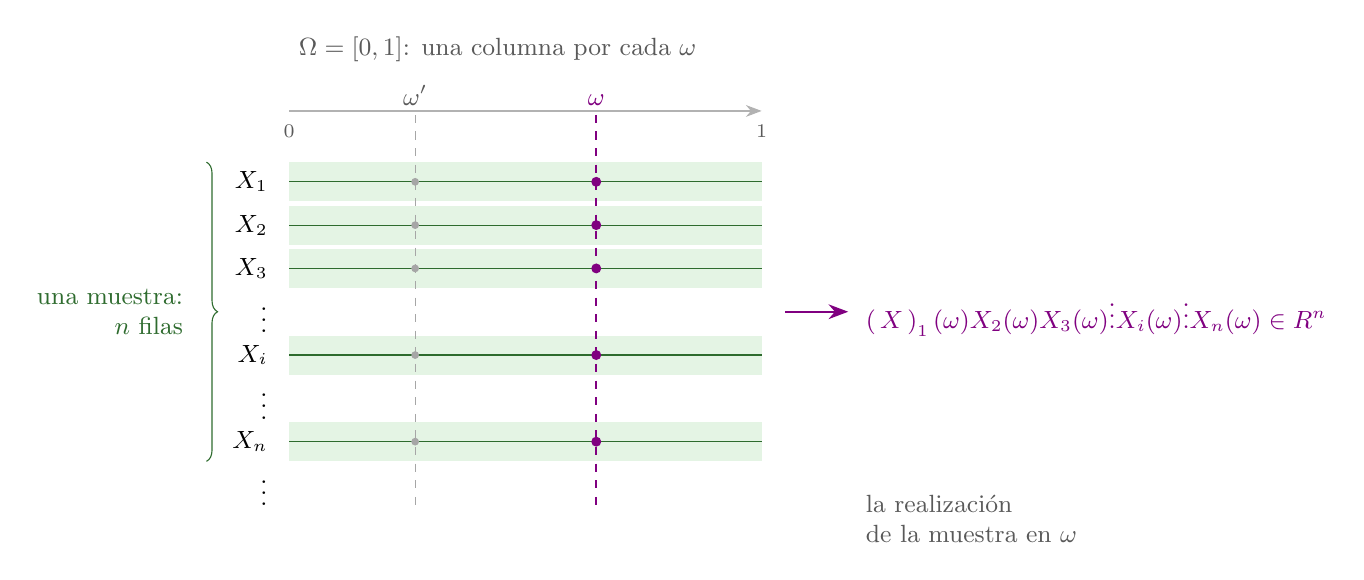
\begin{tikzpicture}[scale=1.0]
    \def\L{6.0}      % anchura de Omega
    \def\h{0.55}     % alto de fila
    \def\om{3.9}     % posición de omega
    \def\omp{1.6}    % otra columna omega'
    % cabecera
    \draw[gray!60,thin,-{Stealth[length=2mm]}] (0,0.35) -- (\L,0.35);
    \node[font=\small,gray!70!black,anchor=south west] at (0,0.85) {$\Omega=[0,1]$: una columna por cada $\omega$};
    \node[font=\scriptsize,gray!70!black,anchor=north] at (0,0.3) {$0$};
    \node[font=\scriptsize,gray!70!black,anchor=north] at (\L,0.3) {$1$};
    % filas: X_1, X_2, X_3, ..., X_i, ..., X_n, ...
    \foreach \k/\lab/\sel in {1/X_1/1, 2/X_2/1, 3/X_3/1, 4/\vdots/0, 5/X_i/1, 6/\vdots/0, 7/X_n/1, 8/\vdots/0}{
      \pgfmathsetmacro{\y}{-\k*\h}
      \ifnum\sel=1
        \fill[\Datos!15] (0,\y-\h*0.45) rectangle (\L,\y+\h*0.45);
        \draw[\Datos!60!black,thin] (0,\y) -- (\L,\y);
      \fi
      \node[font=\small,anchor=east] at (-0.15,\y) {$\lab$};
    }
    % llave de la muestra
    \draw[decorate,decoration={brace,amplitude=4pt,mirror},\Datos!60!black] (-1.05,-7*\h-0.25) -- (-1.05,-1*\h+0.25)
      node[midway,anchor=east,font=\small,align=right,xshift=-5pt,\Datos!60!black] {una muestra:\\ $n$ filas};
    % columna omega
    \draw[\Ajuste,thick,dashed] (\om,0.3) -- (\om,-8.6*\h);
    \node[font=\small,\Ajuste,anchor=south] at (\om,0.3) {$\omega$};
    \foreach \k in {1,2,3,5,7}{ \fill[\Ajuste] (\om,-\k*\h) circle (1.8pt); }
    % otra columna
    \draw[gray!70,thin,dashed] (\omp,0.3) -- (\omp,-8.6*\h);
    \node[font=\small,gray!70!black,anchor=south] at (\omp,0.3) {$\omega'$};
    \foreach \k in {1,2,3,5,7}{ \fill[gray!70] (\omp,-\k*\h) circle (1.4pt); }
    % el vector de R^n
    \draw[-{Stealth[length=2.5mm]},\Ajuste,thick] (\L+0.3,-4*\h) -- (\L+1.1,-4*\h);
    \node[anchor=west,font=\small,\Ajuste] at (\L+1.2,-4*\h) {$\begin{pmatrix}X_1(\omega)\\ X_2(\omega)\\ X_3(\omega)\\ \vdots\\ X_i(\omega)\\ \vdots\\ X_n(\omega)\end{pmatrix}\in\mathbb R^n$};
    \node[anchor=north west,font=\small,gray!70!black,align=left] at (\L+1.2,-8.0*\h) {la realización\\ de la muestra en $\omega$};
  \end{tikzpicture}
\end{document}
